\documentclass{beamer}
\usetheme{AnnArbor}         % tema
\usecolortheme{beaver}      % cores
\mode<presentation>{}
%\documentclass[usenames,dvipsnames]{beamer} % to work around problems with beamer and tikz and beamer and dvipsnames in xcolor package.

\usepackage{multirow}
\usepackage{hyperref}
\usepackage{color}
\usepackage{epsfig}
\usepackage{amsthm}
\usepackage{amssymb}
\usepackage{amsmath}
\usepackage{amscd}
\usepackage[brazilian]{babel}
%\usepackage[utf8]{inputenc}
\usepackage{float}
\usepackage{algpseudocode}
\usepackage{subfig}
\usepackage{listings}
\usepackage{tikz}


\usepackage{times}
\usepackage{multicol}
\usepackage{mathtools}
\usepackage{color}
\usepackage{xcolor} %\usepackage[dvipsnames]{xcolor} % para usar nomes de cores como Fuchsia, Purple, ...
\usepackage{colordvi}
\usepackage{fancyhdr}


% % % % % % % % % % % % % % % % % % % % % % %

% % % % % % % % % % % % % % % % % % % % % % %
\usepackage[OT1]{fontenc}
\usepackage[T1]{fontenc}
\usepackage{amsmath,amsthm,amssymb,enumerate}
\usepackage{stmaryrd}
\usepackage{amsfonts}
\usepackage[]{latexsym}
\usepackage{url}
\usepackage{epigraph}
%\usepackage{anysize}


\usepackage{default}

\usepackage{mathrsfs}  % Para fazer letras como B de Boreliano e F de Filtracao.
\usepackage{esint} % para fazer sinal de integral cortado. - lema de comutadores - livro lions de fluidos vol 1.
\usepackage{textcomp} % para incluir ~ e outros simbolos do Miscellaneous text
\usepackage{wasysym}
%\usepackage[utf8x]{inputenc} % permite usar acentos á é í à ã e outros 



%%%%				  Definitions of parameters     			  %%%%%%%%%%%%%%%%%%%%%%%
%\usetheme{Warsaw}

\setbeamercovered{transparent}

\setbeamertemplate{enumerate items}[default]
\setbeamertemplate{theorems}[ams style]

\definecolor{darkviolet}{rgb}{0.58, 0.0, 0.83}

%\setbeameroption{notes on second screen} % Testar.
%\setbeameroption{show only notes} % useful to print only the notes.
%\setbeameroption{onlyslideswithnotes}
%\setbeameroption{notes on second screen=left} 


% % \setbeamercolor{block body}{fg=blue,bg=white}
% % \setbeamercolor{block body alerted}{fg=blue,bg=white}
% % \setbeamercolor{block body example}{fg=blue,bg=white}


\setbeamertemplate{footline}{} % para tirar footline do beamer
\setbeamertemplate{navigation symbols}{} % para remover os icones de navegacao na parte de baixo da tela.

%\beamertemplatenavigationsymbolsempty
%\setbeamerfont{page number in head/foot}{size=\large}
%\setbeamertemplate{footline}[frame number]


\addtobeamertemplate{navigation symbols}{}{%
	\usebeamerfont{footline}%
	\usebeamercolor[fg]{footline}%
	\hspace{1em}%
	\insertframenumber %/\inserttotalframenumber
}


% % \definecolor{links}{HTML}{2A1B81}
% % \hypersetup{colorlinks,linkcolor=,urlcolor=links}



%% Removes icon in bibliography
%\setbeamertemplate{bibliography item}{}


\setlength{\parindent}{0pt}


\definecolor{darkgreen}{rgb}{0,0.5,0}

% My own definitions of colors 
\definecolor{codegreen}{rgb}{0,0.6,0}
\definecolor{codegray}{rgb}{0.5,0.5,0.5}
\definecolor{codepurple}{rgb}{0.58,0,0.82}
\definecolor{backcolour}{rgb}{0.95,0.95,0.92}

% Definitions on how to display listings
\lstdefinestyle{mystyle}{
	backgroundcolor=\color{white},   
	commentstyle=\color{codegreen},
	keywordstyle=\color{blue},
	numberstyle=\tiny\color{codegray},
	stringstyle=\color{codepurple},
	basicstyle=\tiny,
	language=Python,
	breakatwhitespace=false,         
	breaklines=true,                 
	captionpos= top,%b                    
	keepspaces=true,                 
	numbers=left,                    
	numbersep=5pt,                  
	showspaces=false,                
	showstringspaces=false,
	showtabs=false,
	%stepnumber=3,                  
	tabsize=2
}

\lstset{style=mystyle}

%% Define a new 'leo' style for the package that will use a smaller font.
\makeatletter
\def\url@leostyle{%
	\@ifundefined{selectfont}{\def\UrlFont{\sf}}{\def\UrlFont{\small\ttfamily}}}
\makeatother
%% Now actually use the newly defined style.
\urlstyle{leo}



%%%%%%% New Commands %%%%%%%%%%


% My own definition of size of figures, so that I can change the size of severl figures at once.
\newcommand\sizefigure{0.45} %0.225
\newcommand\szfigrhos{0.45} %0.25
% % % % % % % % % % % % % % % % % % % % % % % % % % % % % % % % 

\newcommand{\gammanikj}[1]{\gamma^{n,#1}_{jl}}
\newcommand{\alphastar}{\alpha^*_j}
\newcommand{\Deltak}[1]{\Delta_{#1}}
\newcommand{\un}[3]{u^{#1}_{n+e_{#2#3}}}
\newcommand{\vecun}{u_n}
\newcommand{\unone}{u_n^1}
\newcommand{\untwo}{u_n^2}
\newcommand{\fracn}{\frac{n_1}{N}}
\newcommand{\fracNn}{\frac{N-n_1}{N}}
\DeclareMathOperator*{\argmin}{arg\,min}
\newcommand{\argminmu}{\argmin\limits_{\mu \in \mathbb{R}^2,~\mu \geq 0}}
\newcommand{\fractions}{\frac{1}{N}(\begin{smallmatrix}n_1\\ N-n_1 \end{smallmatrix})}
\newcommand{\fractionsplus}{\frac{1}{N}(\begin{smallmatrix}n_1+1 \\ N-n_1-1 \end{smallmatrix})}
\newcommand{\fractionsminus}{\frac{1}{N}(\begin{smallmatrix}n_1-1\\ N-n_1+1 \end{smallmatrix})}
\newcommand{\fractionsc}{\frac{n}{N}}
\newcommand{\fractiononetwo}{\frac{n+e_{12}}{N}}
\newcommand{\fractiontwoone}{\frac{n+e_{21}}{N}}
\newcommand{\unoneplus}[1]{u_{n_1+1,N-n_1-1}^{#1}}
\newcommand{\unoneminus}[1]{u_{n_1-1,N-n_1+1}^{#1}}
\newcommand{\unN}[1]{u_{n_1,N-n_1}^{#1}}
\newcommand{\vnN}{v_{n_1,N-n_1}}
\newcommand{\vnNplus}{v_{n_1+1,N-n_1-1}}
\newcommand{\vnNminus}{v_{n_1-1,N-n_1+1}}
\newcommand{\vecvone}{(\begin{smallmatrix} 0 \\ -\vnN\end{smallmatrix})}
\newcommand{\vecvtwo}{(\begin{smallmatrix} \vnN \\ 0\end{smallmatrix})}
\newcommand{\vecvonem}{(\begin{smallmatrix} 0 \\ -v_{n_1-1,N-n_1+1}\end{smallmatrix})}
\newcommand{\vecvtwop}{(\begin{smallmatrix} v_{n_1+1,N-n_1-1} \\ 0\end{smallmatrix})}
\newcommand{\vn}{v_n}

\newcommand{\Rr}{{\mathbb{R}}}
\newcommand{\Nn}{{\mathbb{N}}}
\newcommand{\ej}{{e_j}}
\newcommand{\ek}{{e_k}}
\newcommand{\ejk}{{e_{jk}}}
\newcommand{\ekj}{{e_{kj}}}

\newcommand{\trace}{\operatorname{trace}}
\newcommand{\argmax}{\operatorname{argmax}}
\renewcommand{\div}{\operatorname{div}}
\newcommand{\osc}{\operatorname{osc}}
\newcommand{\Ll}{{\mathcal{L}}}
\newcommand{\Aaa}{{\mathcal{A}}}
\newcommand{\Tt}{{\mathbb{T}}}
\newcommand{\E}{\mathbb E}
\newcommand{\Ii}{\mathcal I}
\newcommand{\PP}{\mathbb P}
\newcommand{\Pp}{\mathcal P}
\newcommand{\mS}{\mathbb S}
\newcommand{\cH}{\mathcal H}
\newcommand{\cD}{\mathcal D}
\newcommand{\cT}{\mathcal T}
\newcommand{\cG}{\mathcal G}
\newcommand{\cU}{\mathcal U}
\newcommand{\cL}{\mathcal L}
\newcommand{\cM}{\mathcal M}
\newcommand{\cN}{\mathcal N}
\newcommand{\bq}{\mathbf{q}}
\newcommand{\hH}{\hat{H}}
\newcommand{\bG}{\bar{G}}
\newcommand{\Hh}{\bar{H}}
\newcommand{\bL}{\bar{L}}
\newcommand{\tH}{\tilde{H}}
\newcommand{\af}{\alpha}
\newcommand{\fui}{\varphi}
\newcommand{\ep}{\epsilon}
\newcommand{\be}{\beta}
\newcommand{\ga}{\gamma}
\newcommand{\Ga}{\Gamma}
\newcommand{\de}{\delta}
\newcommand{\om}{\omega}
\newcommand{\lam}{\lambda}
\newcommand{\te}{\theta}
\newcommand{\lV}{\left\Vert}
\newcommand{\rV}{\right\Vert}
\newcommand{\rip}{\rangle}
\newcommand{\lip}{\langle}
\newcommand{\mL}{\mathbb L}
\newcommand{\mH}{\mathbb H}
\newcommand{\Ff}{\mathbb F}

\renewcommand{\div}{\operatorname{div}}
\newcommand{\diver}{\operatorname{div}}
\newcommand{\rot}{\operatorname{rot}}
\newcommand{\flux}{\operatorname{flux}}
\newcommand{\lap}{\bigtriangleup}
\newcommand{\dom}{\operatorname{dom}}
\newcommand{\sgn}{\operatorname{sgn}}
\newcommand{\hes}{\operatorname{Hess}}
\newcommand{\Alt}{\operatorname{Alt}}
\newcommand{\entre}{\setminus}
\newcommand{\ann}{\operatorname{ann}}
\newcommand{\graf}{\operatorname{graph}}
\newcommand{\pr}{\operatorname{proj}}
\newcommand{\tr}{\operatorname{Tr}}
\newcommand{\sop}{\operatorname{supp}}
\newcommand{\dHp}{\dfrac{\partial H}{\partial p}}

\newcommand{\bx}{{\bf x}}
\newcommand{\bu}{{\bf u}}
\newcommand{\bdu}{\dot {\bf u}}
\newcommand{\bdx}{\dot{\bf x}}
\newcommand{\bddx}{\ddot{\bf x}}
\newcommand{\bp}{{\bf p}}
\newcommand{\bdp}{\dot{\bf p}}
\newcommand{\br}{{\bf r}}
\newcommand{\bdr}{\dot{\bf r}}
\newcommand{\bX}{{\bf X}}
\newcommand{\bdX}{\dot{\bf X}}
\newcommand{\bY}{{\bf Y}}
\newcommand{\bdY}{\dot{\bf Y}}
\newcommand{\bP}{{\bf P}}
\newcommand{\bdP}{\dot{\bf P}}
\newcommand{\by}{{\bf y}}
\newcommand{\bdy}{\dot{\bf y}}
\newcommand{\bv}{{\bf v}}
\newcommand{\bdv}{\dot{\bf v}}
\newcommand{\bw}{{\bf w}}
\newcommand{\bdw}{\dot{\bf w}}
\newcommand{\bz}{{\bf z}}
\newcommand{\bdz}{\dot{\bf z}}

\newcommand{\bi}{{\bold{i}}}
\newcommand{\bj}{{\bold{j}}}
\newcommand{\bk}{{\bold{k}}}
\newcommand{\bn}{{\bold{n}}}
\newcommand{\bom}{{\bold{m}}}


 %%%%%%%%%%%%%%%%%%%%%%%%%%%%%%%%%%%%%%%%%%%%
\newcommand{\N}{{\mathbb N}}  \newcommand{\R}{{\mathbb R}}  \newcommand{\RN}{{{\mathbb R}^N}}  \newcommand{\C}{{\mathbb C}}
\newcommand{\glnc}{GL_{n}(\mathbb C)}  \newcommand{\CP}{{\mathbb C \mathbb P}}
\newcommand{\ds}{\displaystyle}  \newcommand{\nl}{\newline}
\newcommand{\Lploc}{{L_{loc}^p}}
\newcommand{\eps}{{\varepsilon}}
\newcommand{\seq}{seq\"u\^encia}
\newcommand{\ud}{\,\mathrm{d}}
\newcommand{\intRN}{{\underset{{{\mathbb R}^N}}{\int}}}
\newcommand{\eq}{{equa\c c\~ ao }} \newcommand{\Eq}{{Equa\c c\~ ao }} \newcommand{\fnc}{{fun\c c\~ ao }} \newcommand{\sol}{{solu\c c\~ ao }}
\newcommand{\cao}{{\c c\~ ao }} \newcommand{\coes}{{\c c\~ oes }}
\newcommand{\dive}{\nabla \cdotp}
%%%%%%%%%%%%%%%%%%%%%%%%%%%%%%%%%%%%%%%%%%%%%


\algnewcommand{\LineComment}[1]{\State \(\triangleright\) #1}
\def  \R   {{\mathbb R}}
\def  \Z   {{\mathbb Z}}
%\def  \N   {{\mathbb N}}
\def  \Q   {{\mathbb Q}}
\def \Ev {{\mathbb E}}
\def \Pr {{\mathbb P}}
\def \f {{\mathbf f}}
\def \u {{\mathbf u}}
\def \y {{\mathbf y}}
\def \x {{\mathbf x}}
\def \m {{\mathbf m}}
\def \gu {{\bar{g}}}

\newcommand{\Var}{\mathrm{Var}}
\newcommand{\Cov}{\mathrm{Cov}}
%%%%%%%%%%%%%%%%%%%%%%%%%%%%%%%%%

\newtheorem{proposition}[theorem]{Proposi\c c\~ ao}

\renewcommand{\definition}{\definicao}
\newtheorem{definicao}[theorem]{Defini\c c\~ ao}

\renewcommand{\corollary}{\corolario}
\newtheorem{corolario}[theorem]{Corol\' ario}



%%%%%%%%%%%%%%%%%%%%%%%%%%%%%%%%%%%%%%%%%%%%%%%%%%%%%%%%%%%%%%%%%%%%%%%
\title{Variational Inference and Bayesian Monte Carlo}
\author[Danilo Naiff]{{{\bf \large Danilo de Freitas Naiff} \vspace{0.75cm} \\{\bf NIDF-UFRJ}} \\ \vspace{0.8cm}}
%\institute{\Large AIMS 2016 - Orlando}
\date{Oct. 18nd 2019}


%%%%%%%%%%%%%%%%%%%%%%%%%%%%%%%%%%%%%%%%%%%%%%%%%%%%%%%%%%%%%%%%%%%%%%%%%%%%%%%%%%%%%%%%%%%%%%%%%%%%%%%%%%%%%%%


\begin{document}
	\frame{\titlepage}


\section*{Outline}
\begin{frame}{}\tableofcontents
\end{frame}

%% normal frame
\section{Introduction}

\begin{frame}{}
\begin{block}{Bayesian theory}
Objective: update knowledge of parameter $\theta$ given data $\mathcal{D}$.
\pause

Probabilistic model $M$
\begin{itemize}
\item Prior probability $p(\theta)$
\item Likelihood $p(\mathcal{D}|\theta)$
\end{itemize}
\pause
Posterior probability
\begin{equation*}
p(\mathcal{\theta}|\mathcal{D}) = \frac{p(\mathcal{D}|\theta) p(\theta)}{\int p(\mathcal{D}|\theta') p(\theta') d \theta'}
\end{equation*}
\pause
Using posterior probability:
\begin{equation*}
\langle f(\theta) \rangle = \int_\Theta f(\theta) p(\theta|\mathcal{D}) d \theta
\end{equation*}
\end{block}
\end{frame}

\begin{frame}{}
\begin{block}{Bayesian decision theory}
To use posterior probabilities to make decisions, formally one requires a loss function $L : \Theta \times \mathcal{A} \to \mathbb{R}^+$. Optimal decision:
\begin{equation*}\label{generalloss}
a^* = \argmin_{a \in \mathcal{A}} \int_\Theta L(\theta,a) p(\theta|\mathcal{D},M) d \theta,
\end{equation*}
Considering estimation as decision:
\begin{equation*}
\hat{\theta} = \argmin_{\tilde{\theta}} \int L(\theta,\tilde{\theta}) p(\theta|\mathcal{D},M) d \theta
\end{equation*}
For some losses:
\begin{itemize}
	\item The $l_2$ (quadratic) loss $L(\theta,\tilde{\theta}) = ||\theta - \tilde{\theta}||_2^2$, for which $\hat{\theta} = \Ev[\theta|\mathcal{D},M]$
	\item The $l_1$ (absolute) loss $L(\theta,\tilde{\theta}) = ||\theta - \tilde{\theta}||_1$, for which, at each coordinate $i$, $\hat{\theta}_i = \text{median}(\theta_i|\mathcal{D},M)$.
\end{itemize}
\end{block}
\end{frame}
\begin{frame}{}
\begin{block}{Model selection}
Obviously, we don't know in principle which model is correct. So we must choose between models.
\begin{equation*}\label{modelselectionobjective}
\hat{M} = \argmax_{M \in \mathcal{M}} p(\mathcal{D} | M) = \argmax_{M \in \mathcal{M}} \int p(\mathcal{D} | \theta_M, M) p(\theta_M | M) d\theta_M.
\end{equation*}
Model selection in Bayesian theory is interesting, since it displays the Occam's razor effect.
\end{block}
\end{frame}

\begin{frame}{}
\begin{block}{Approximate inference}
Ways to integrate:
\begin{itemize}
\item Monte Carlo
\begin{equation*}
\int_\Theta f(\theta) p(\theta|\mathcal{D}) d\theta \approx \frac{1}{N} \sum_{i=1}^N f(\theta_i), \quad \theta_i \sim p(\theta|\mathcal{D})
\end{equation*}
\item Approximate distribution
\begin{equation*}
p(\theta|\mathcal{D}) \approx q(\theta), \quad \langle f(\theta) \rangle \approx \int_\Theta f(\theta) q(\theta) d\theta
\end{equation*}
\end{itemize}

\end{block}
\end{frame}

\section{Variational Inference}
\begin{frame}{}
\begin{block}{Approximating posteriors}
	\begin{equation*}
	p(\theta|\mathcal{D}) = g(\theta) \approx q(\theta;\lambda)
	\end{equation*}
	Choosing $q$: minimizing some measure of dissimilarity. The family $q(\theta;\lambda)$ must be easy to treat, in order for the approximation to be useful.
	
	Variational inference: uses $D_{KL}(q(\cdot;\lambda)||g)$ for measure of dissimilarity
	\begin{equation*}
	D_{KL}(q||g) = -\int \log \frac{p(\theta)}{q(\theta)} q(\theta) d\theta
	\end{equation*}
	
\end{block}
\begin{block}{$D_{KL}(q||g)$ vs $D_{KL}(g||q)$}
	$D_{KL}(q||g) \geq 0$, $D_{KL}(q||g) = 0 \iff q=g$, but $D_{KL}(q||g) \neq D_{KL}(g||q)$. 
	Then, KL divergence minimization gives two different algorithms, the second one being \textit{expectation propagation}.
	
\end{block}
\end{frame}

\begin{frame}{}
\begin{block}{Illustration}
\begin{figure}
	\centering
	\captionsetup[subfigure]{labelformat=empty}
	\subfloat[$D_{KL}(q||g)$ ]{\label{vixep1a}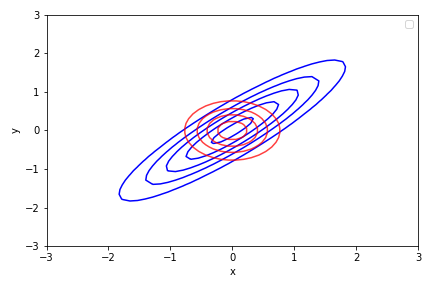
\includegraphics[width=0.45\textwidth]
		{figs/klil3a.png}}
	\subfloat[$D_{KL}(g||q)$]{\label{vixep1b}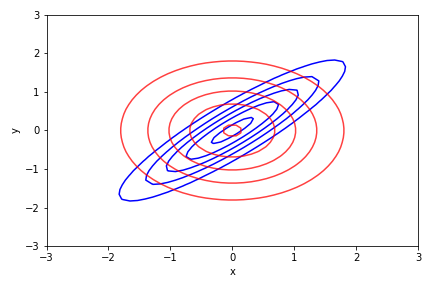
\includegraphics[width=0.45\textwidth]
		{figs/klil3b.png}}
\end{figure}
\end{block}
\end{frame}

\begin{frame}{}
\begin{block}{Evidence lower bound}
Usually, one only has access to $p(\mathcal{D}|\theta) p(\theta) = \gu(\theta)$. Fortunately, minimizing $D_{KL}(q||g)$ is equivalent to maximizing the \textit{evidence lower bound} (ELBO).

\begin{equation*}
\mathcal{L}_\gu(q) = 
\int \log \gu(\theta) q(\theta) d\theta - \int \log q(\theta) q(\theta) d\theta
\end{equation*}
\end{block}{}
\begin{block}{Model selection using ELBO}
\begin{equation*}
\begin{split}
\log p(\mathcal{D}) & = \log \Ev_{\theta \sim p(\theta)} [p(\mathcal{D}|\theta)] \\
& = \log \Ev_{\theta \sim q(\theta)} \left[\frac{p(\mathcal{D}|\theta) p(\theta)}{q(\theta)} \right] \\
& \geq \Ev_{\theta \sim q(\theta)} \left[ \log \frac{p(\mathcal{D}|\theta) p(\theta)}{q(\theta)} \right] = \mathcal{L}(q).
\end{split}
\end{equation*}
Moreover, $\mathcal{L}_\gu(q) \leq \log p(\mathcal{D})$. Can be used for model selection.
\end{block}
\end{frame}
\begin{frame}
\begin{block}{Maximizing the ELBO}
For parameterized $q(\theta;\lambda)$: access to stochastic estimation of $\nabla \mathcal{L}(\lambda)$ can be used for stochastic gradient ascent.
\end{block}
\begin{block}{REINFORCE}
\begin{equation*}\label{reinforce}
\nabla \mathcal{L}(\lambda) = \Ev_{\theta \sim q(\theta;\lambda)} \left[ \log \frac{\gu(\theta)}{q(\theta;\lambda)} \nabla_{\lambda} \log q(\theta;\lambda) \right], 
\end{equation*}
Approximation by Monte Carlo estimator. 
\begin{equation*}\label{reinforcemc}
\nabla \mathcal{L}(\lambda) \approx \frac{1}{K} \sum_{i \in [K], \theta_i \sim q(\theta;\lambda)} \log \frac{\gu(\theta_i)}{q(\theta_i;\lambda)} \nabla_{\lambda} \log q(\theta_i;\lambda),
\end{equation*}
One option for controlling high variance:
\begin{equation*}
\Ev_{\theta \sim q(\theta;\lambda)} \left[ \left( \log \left( \frac{\gu(\theta)}{q(\theta;\lambda)}\right) + C\right) \nabla_{\lambda} \log q(\theta;\lambda) \right], 
\end{equation*}
\end{block}
\end{frame}
\begin{frame}{}
\begin{block}{Reparameterization}
Reparametrization: if samples $X_\lambda \sim q(\theta;\lambda)$ can be writen as $s(Y,\lambda)$, with $Y \sim r(\epsilon)$:

$\nabla \mathcal{L}(\lambda) = \nabla \left( \Ev_{r(\epsilon)} \left[\log \frac{ \gu(s(\epsilon;\lambda))}{q(s(\epsilon;\lambda);\lambda)}\right]\right) \approx \frac{1}{K} \sum_{Y_i \sim r(\epsilon)} \nabla \left( \log \frac{ \gu(s(Y_i;\lambda))}{q(s(Y_i;\lambda);\lambda)} \right).$
\end{block}
\begin{block}{Possible distributions for reparamaterization}
Distributions that can be used for reparameterization:
\begin{itemize}
	\item Tractable inverse CDF. Examples: Exponential, Cauchy, Logistic, Rayleigh, Pareto, Weibull, Reciprocal,Gompertz, Gumbel, Erlang and Kumaraswamy distributions.
	\item Location-scale families. Examples: Gaussian, Laplace, Elliptical, Student's t, Uniform.
	\item Compositions. Examples: Log-normal, Chi-squared
\end{itemize}
\end{block}
\end{frame}
\begin{frame}{}
\begin{block}{Reparameterization x REINFORCE}
\begin{figure}[h]
	\centering
	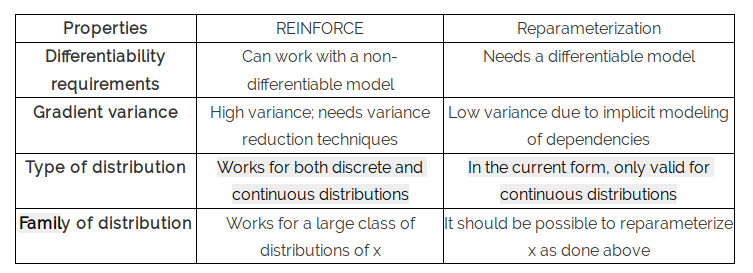
\includegraphics[height=.35\linewidth]{figs/reinforce_x_reparameterization.png}
	%\includegraphics[height=6cm]{figCoordEsf02}
\end{figure}
Source: \url{http://stillbreeze.github.io/REINFORCE-vs-Reparameterization-trick/}.
\end{block}
\end{frame}
\begin{frame}{}
\begin{block}{Mixture of Gaussians}
$q_k(\theta;\lambda) = \sum_{i=1}^k w_i f_i(\theta) = \sum_{i=1}^k w_i \mathcal{N}(\theta;\mu_,\Sigma_i)$. Analytical mean and covariance. Samples can be easily generated. Are in a sense universal approximators. \text{Good choice for variational approximation}.
\end{block}
\begin{block}{Parameterizing mixtures of Gaussian}
Covariance parameterizations: 
\begin{itemize}
\item $\Sigma_i = \text{diag}(\sigma_{i,1}^2,\ldots,\sigma_{i,D}^2)$
\item $\Sigma_i = \u_i \u_i^T + \text{diag}(\sigma_{i,1}^2,\ldots,\sigma_{i,D}^2)$
\end{itemize}

Weights parameterizations $w_i(\nu_i) = \frac{\phi(\nu_i)}{\sum_{i=1}^k \phi(\nu_k)}$. $\phi(\nu)$ can be $\exp(\nu)$ or $\text{softplus}(\nu) = \log(1+\exp(\nu))$
\end{block}
\begin{block}{ELBO for mixtures of Gaussians}
\begin{equation*}
\mathcal{L}(\lambda) = \sum_{i=1}^k w_i(\nu_i) \Ev_{\epsilon \sim \mathcal{N}(0,I)}\left[\log \frac{ \gu(s(\epsilon;\mu_i,\sigma_i))}{q_k(s(\epsilon;\mu_i,\sigma_i);\lambda)}\right]
\end{equation*}
\end{block}
\end{frame}

\begin{frame}{}
\begin{block}{Boosting mixtures}
Problem: no way to know how many mixtures is needed. Adding mixtures sequentially can become costly. One solution: boosting.
$q_{i-1}(\theta) = \sum_{j=1}^{i-1} w_j f_j(\theta)$

$q_{i}(\theta) = \sum_{j=1}^{i-1} (1-w_{i}) w_j f_j(\theta) + w_{i} f_i(\theta)$

How to find $w_{i}$ and $f_i(\theta) = \mathcal{N}(\theta;\mu_{i},\Sigma_{i})$?
\end{block}
\begin{block}{Setting component weights}
Given component $f_i(\theta)$, maximize 
$\mathcal{L}_i(w_i) = \mathcal{L}((1-w_{i}) q_{i-1}(\theta) + w_{i} f_i(\theta))$
via its derivative
\begin{equation*}
\begin{split}
\mathcal{L}'_{i}(w_{i}) & = \int \log (\gu(\theta)) (f_{i}(\theta) - q_{i-1}(\theta)) d\theta - \\
& \qquad{} \int \log((1-w_{i}) q_{i-1}(\theta) + w_{i} f_{i}(\theta)) (f_i(\theta) - q_{i-1}(\theta)) d\theta.
\end{split}
\end{equation*}
Fortunately, $\mathcal{L}_i(w_i)$ is a concave objective.
\end{block}
\end{frame}

\begin{frame}{}
\begin{block}{Finding components}
Gradient boosting: technique for finding new components.
\begin{equation*}
\begin{split}
f_i = \argmin_{f} \nabla D_{KL}(q_{i-1} || g) \cdot f = \argmin_{f} \int \log \frac{q_{i-1}(\theta)}{g(\theta)} f(\theta) d\theta.
\end{split}
\end{equation*}
Problem: degenerate solution. Needs regularization.

Maximization objective for mixture of Gaussians:
\begin{equation*}
\begin{split}
\text{RELBO}(\mu_i,\Sigma_i) = & \int \log(\gu(\theta)) \mathcal{N}(\theta|\mu_i,\Sigma_i) d\theta - \\
& \int \log(q_{i-1}(\theta)) \mathcal{N}(\theta|\mu_i,\Sigma_i) d\theta + \frac{\lambda}{4} \log |\Sigma|,
\end{split}
\end{equation*}
Reparameterization trick can be used.
\end{block}

\end{frame}

\begin{frame}{}
\begin{figure}
\begin{algorithmic}[1]\label{vbalgorithm}
\Procedure{VariationalBoosting}{$\log \gu,\mu_0$,$\Sigma_0$}
\LineComment{$\mu_0,\Sigma_0$ the are initial boosting values}
\State $w_0 := 1.0$
\For{$t=1,...,T$}
\State $\mu_{t},\Sigma_{t} := \argmax RELBO(\mu_{t},\Sigma_{t})$ \Comment{Using reparameterization}
\State $w_{t} := \argmax \mathcal{L}_i(w_i)$ \Comment{Using $\mathcal{L}'_t(w_t)$ for gradient descent}
\For{$j=0,...,t-1$}
\State $w_{j} \gets (1-w_t)w_j$
\EndFor
\EndFor
\State \Return $\{(\mu_t,\Sigma_t,w_t)\}_{t=1}^T$
\EndProcedure
\end{algorithmic}
\end{figure}
\end{frame}

\begin{frame}
\begin{block}{}
In science, there are many cases that $p(\mathcal{D}|\theta)$ demands the computation of a forward model $g(\theta)$, which comes from an expensive simulation.
\begin{figure}[h]
\centering
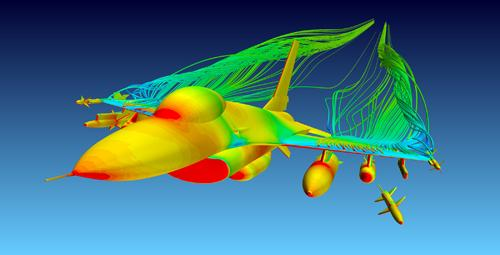
\includegraphics[height=0.3\paperheight]{figs/simulation_figure.jpg}
%\includegraphics[height=6cm]{figCoordEsf02}
\end{figure}
\pause
This requires approximate inference methods "on a budget". In this work, one such method is developed, based on preexisting work. We name it
\pause 
\begin{block}{}
\centering{\textit{Boosted Variational Bayesian Monte Carlo (BVBMC)}.}
\end{block}
\end{block}
\end{frame}

\begin{frame}{}
\begin{block}{BVBMC schema}
\begin{figure}[h]
\centering
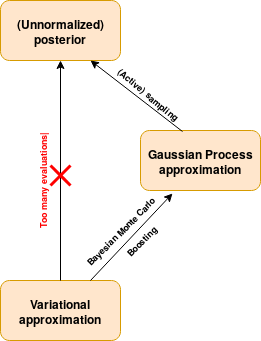
\includegraphics[height=.5\linewidth]{figs/diagram1a.png}
%\includegraphics[height=6cm]{figCoordEsf02}
\end{figure}
\end{block}
\end{frame}

\begin{frame}{}
\begin{block}{An illustration of BVBMC}
\centering{
\begin{tikzpicture}
\node<1> (exfig1) {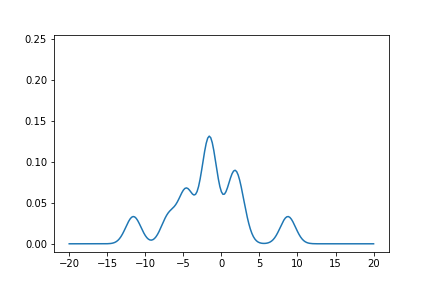
\includegraphics[width=.7\linewidth]{figs/exampleintro1}};
\node<2> (exfig2) {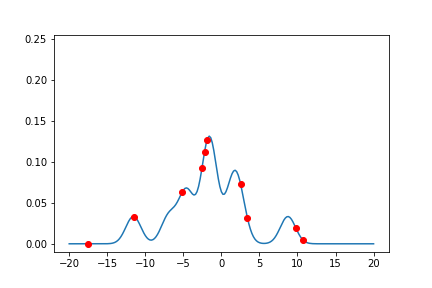
\includegraphics[width=.7\linewidth]{figs/exampleintro2}};
\node<3> (exfig3) {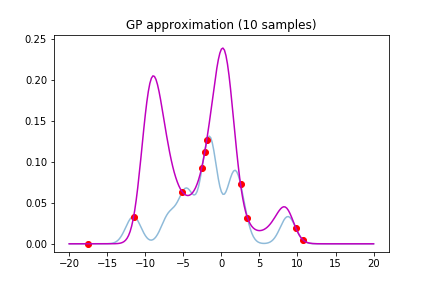
\includegraphics[width=.7\linewidth]{figs/exampleintro3}};
\node<4> (exfig3) {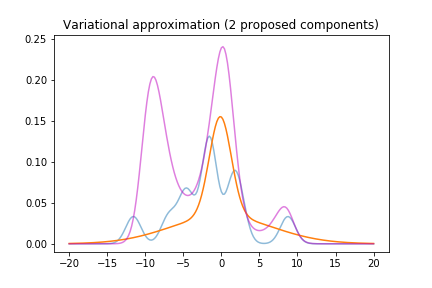
\includegraphics[width=.7\linewidth]{figs/exampleintro4}};
\node<5> (exfig3) {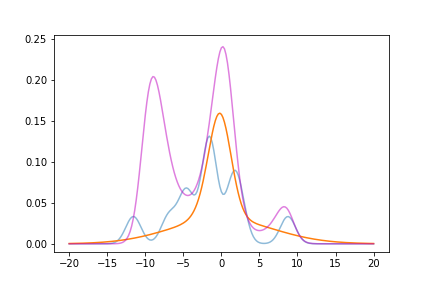
\includegraphics[width=.7\linewidth]{figs/exampleintro5}};
\node<6> (exfig3) {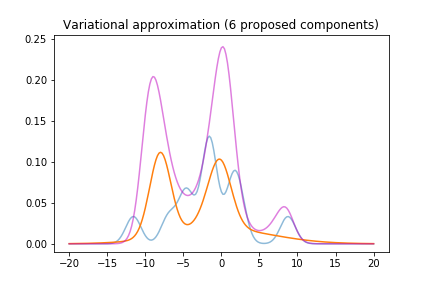
\includegraphics[width=.7\linewidth]{figs/exampleintro6}};
\node<7> (exfig3) {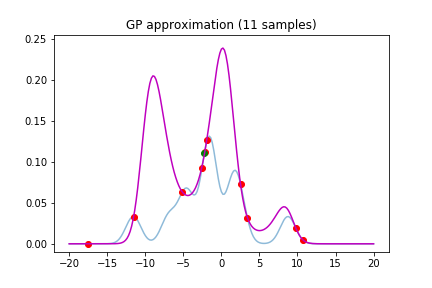
\includegraphics[width=.7\linewidth]{figs/exampleintro7}};
\node<8> (exfig3) {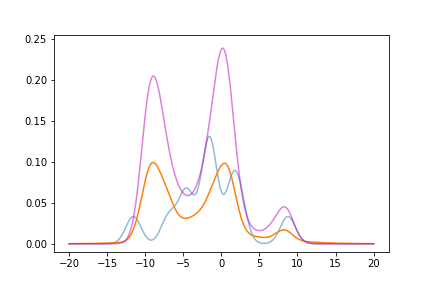
\includegraphics[width=.7\linewidth]{figs/exampleintro8}};
\node<9> (exfig3) {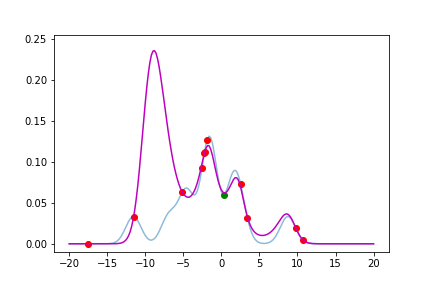
\includegraphics[width=.7\linewidth]{figs/exampleintro9}};
\node<10> (exfig3) {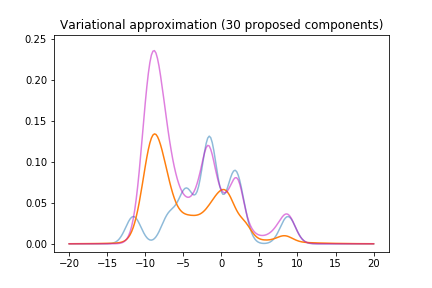
\includegraphics[width=.7\linewidth]{figs/exampleintro10}};
\node<11> (exfig3) {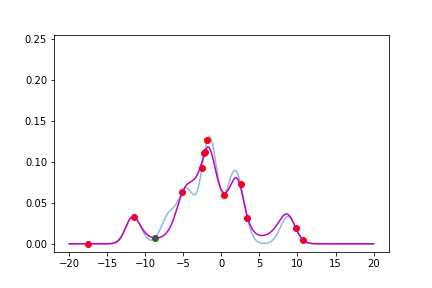
\includegraphics[width=.7\linewidth]{figs/exampleintro11}};
\node<12> (exfig3) {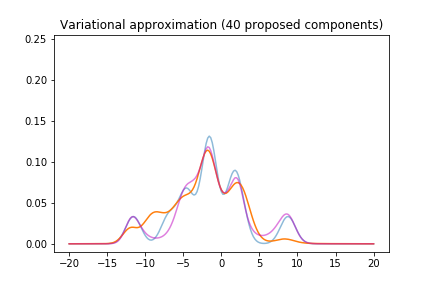
\includegraphics[width=.7\linewidth]{figs/exampleintro12}};
\node<13> (exfig3) {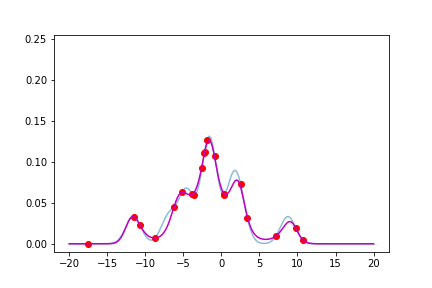
\includegraphics[width=.7\linewidth]{figs/exampleintro13}};
\node<14> (exfig3) {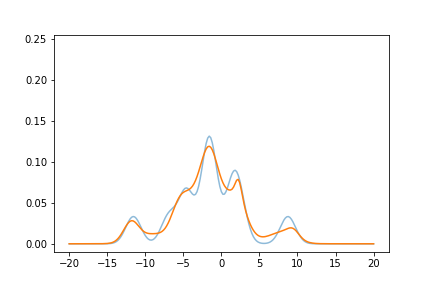
\includegraphics[width=.7\linewidth]{figs/exampleintro14}};

\end{tikzpicture}
}
\end{block}
\end{frame}

\section{Gaussian Processes}
\begin{frame}{}
\begin{block}{Definition}
Gaussian processes (GP): distribution over functions $f:\mathcal{X} \to \mathbb{R}$ such that $f(\mathbf{x}) = (f(x_1),\ldots,f(x_n))$ follows a multivariate normal distribution. A GP is completely defined by:
\begin{itemize}
\item $m(x;\theta) := \Ev[f(x)]$, mean function.
\item $k(x,x';\theta) := \Cov[f(x),f(x')]$, covariance function or kernel.
\end{itemize}
such that $f(\mathbf{x}) \sim \mathcal{N}(m(\mathbf{x}),K(\mathbf{x},\mathbf{x}))$.
\end{block}
%\pause
\begin{block}{Gaussian process regression}
Given $\mathcal{D} = {(x,y)}_{i=1}^N$, a Gaussian process regression is made by assuming $p(y|x) = p(y|f(x))$, with $f$ following a prior $GP(m,k)$.
\end{block}

\end{frame}

\begin{frame}{}
\begin{block}{Posterior GP}
If $p(y|f(x)) = \mathcal{N}(f(x),\sigma_n^2)$, $f|\mathcal{D} \sim GP(m_\mathcal{D},k_\mathcal{D})$, where 
\begin{equation*}
\begin{split}
m_\mathcal{D}(x) & := m(x) + K(x^\star,\mathbf{x}) (K(\mathbf{x},\mathbf{x})+\sigma^2_n I)^{-1} (\mathbf{y} - m(\mathbf{x})) \\
k_\mathcal{D}(x,x') & := k(x,x') - K(x,\mathbf{x})(K(\mathbf{x},\mathbf{x})+\sigma_n^2 I)^{-1}K(\mathbf{x},x)
\end{split}
\end{equation*}
Reduces to deterministic measurement when $\sigma_n^2 = 0$. More general $p(y|f(x))$ must resort to explicit marginalization.
\end{block}
\end{frame}

\begin{frame}{}
\begin{block}{Example case}


\begin{figure}
\centering
\captionsetup[subfigure]{labelformat=empty}
\subfloat[GP prior]{\label{gprex1a}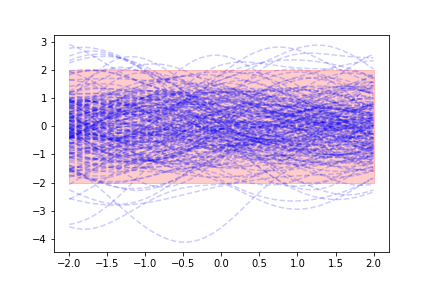
\includegraphics[width=0.5\textwidth]
{figs/gprex1a.png}}
\subfloat[GP posterior]{\label{gprex1b}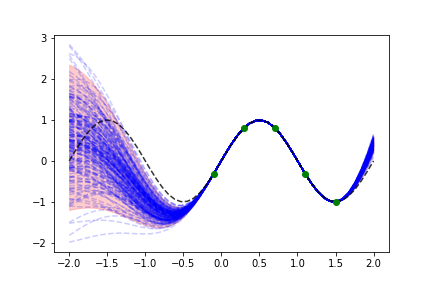
\includegraphics[width=0.5\textwidth]
{figs/gprex1b.png}}

\end{figure}

\end{block}
\end{frame}

\begin{frame}{}
\begin{block}{Kernels}
The assumption that $K(\mathbf{x},\mathbf{x})$ is a covariance matrix restricts which functions can be kernels. Some examples of kernels in $\mathbb{R}$ are:
\begin{itemize}
\item $k_{SQE}(x,x';\theta_0,l) = \theta_0 \exp \left(-\frac{1}{2} \frac{(x-x')^2}{l^2} \right)$
\item $k_{\text{Matern},3/2}(x,x';\theta_0,l) = \theta_0 \left( \sqrt{3} \frac{(x-x')}{l} \right) \exp \left(-\sqrt{3} \frac{(x-x')}{l}\right)$
\end{itemize}
Kernels in $\mathbb{R}^D$ can be constructed by changing $\frac{(x-x')}{l}$ for $\sqrt{\sum_{i=1}^D \frac{(x_i-x_i')}{l_i}}$.

If $k_1$,$k_2$ are kernels, the following, among others are kernels: $k_1(x,x')+k_2(x,x')$,$k_1(x,x')k_2(x,x')$,$k_1(x,x')k_2(y,y')$,$k_1(f(y),f(y'))$.
\end{block}
%\pause
\begin{block}{Mean functions}
In general,they are less important than kernels, since the latter determines the structure of the posterior GP. However, \textit{outside the sampling area the GP prediction defaults to the mean}, which may be of importance.
\end{block}
\end{frame}

\begin{frame}{}
\begin{block}{Handling hyperparameters}
\begin{equation*}
\begin{split}
\log p(\mathcal{D}|\theta) = & -\frac{1}{2}(\mathbf{y} - m(\mathbf{x}))^T (K(\mathbf{x},\mathbf{x}) + \sigma_n \mathbf{I})^{-1} (\mathbf{y} - m(\mathbf{x})) + \\
&-\frac{1}{2} \log \det (K(\mathbf{x},\mathbf{x}) + \sigma_n \mathbf{I}) - \frac{1}{2} N \log(2\pi).
\end{split}
\end{equation*}
Inference can be done either by MLE, MAP, or integration techniques.
\end{block}
\begin{block}{Scaling}
The bottleneck of GP regression: $(K(\mathbf{x},\mathbf{x}) + \sigma_n \mathbf{I})^{-1}$. Cost is $\mathcal{O}(N^3)$.

In online learning, each new sample is incorporated in $\mathcal{O}(N^2)$.
\end{block}

\end{frame}

\section{Bayesian Monte Carlo}
\begin{frame}{}
\begin{block}{Integrating a GP}
As discussed, often one wants to take expectations
\begin{equation*}
Z = \int f(x) p(x) dx
\end{equation*}
Bayesian Monte Carlo: given $\mathcal{D} = \{x_i,f(x_i)\}_{i=1}^N$, approximate $f$ by $f_\mathcal{D} \sim GP(m_\mathcal{D},k_\mathcal{D})$. This makes
\begin{equation*}
Z_\mathcal{D} = \int f_\mathcal{D}(x) p(x) dx
\end{equation*}
be a Gaussian random variable

%\pause
\begin{block}{}
\centering{Name Bayesian \textit{Monte Carlo} is misleading.}
%\pause

\end{block}
\end{block}
\end{frame}
\begin{frame}{}
\begin{figure}
\centering
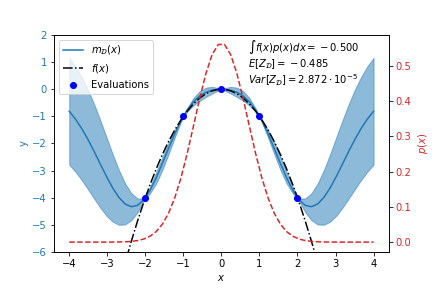
\includegraphics[width=0.8\linewidth]{figs/exbmc.png}
\end{figure}
\end{frame}
\begin{frame}{}
\begin{block}{Mean and variance for BMC}
\begin{equation*}
\begin{split}
& \Ev[Z_{\mathcal{D}}] = \int m(x) p(x) dx - \mathbf{z}^T K^{-1} (\mathbf{f}-m(\mathbf{x})), \quad
\Var[Z_{\mathcal{D}}] = \Gamma - \mathbf{z}^T K^{-1} \mathbf{z}, \\
& z_i = \int k(x,x_i) p(x) dx, \quad \Gamma = \int \int k(x,x') p(x) p(x') dx dx'.
\end{split}
\end{equation*}
\end{block}
\begin{block}{Kernel integral terms}
In the general case, they can be estimated by Monte Carlo.
When $p(x)$ is Gaussian or a mixture of Gaussians:
\begin{itemize}
\item Analytically tractable when $k(x,x')$ is the SQE kernel.
\item Efficiently tractable when $k(x,x') = k(x_1,y_1) \ldots k(x_D,y_D)$.
\end{itemize}
\end{block}
\end{frame}
\begin{frame}
\begin{block}{Active evaluation}
Given $\{(x_1,f(x_1)),\ldots,(x_N,f(x_N))\}$, $x_{N+1}$ may be chosen by maximizing \textit{acquisition functions}.
\begin{equation*}
\alpha^N(x) = \alpha(x;\{(x_1,f(x_1)),\ldots,(x_N,f(x_N))\})
\end{equation*}
Examples:
\begin{itemize}
\item For general integrands
\begin{equation*}
\alpha^N_{\text{US}}(x) = k_\mathcal{D}(x,x) p(x)^2
\end{equation*}
\item For positive integrands
\begin{equation*}
\alpha^N_{\text{MMLT}}(x) = e^{2 m_\mathcal{D}(x) + k_\mathcal{D}(x,x)} \left(e^{k_\mathcal{D}(x,x)}-1\right).
\end{equation*}
\end{itemize}
\end{block}
\end{frame}


\begin{frame}{}
\begin{block}{Variational Bayesian Monte Carlo (VBMC)}
$\mathcal{L}(\lambda) = 
\int \log \gu(\theta) q(\theta;\lambda) d\theta - \int \log q(\theta;\lambda) q(\theta;\lambda) d\theta$

Use Bayesian Monte Carlo:
$\mathcal{L}_\mathcal{D}(\lambda) = 
\int \log \gu_\mathcal{D}(\theta) q(\theta;\lambda) d\theta - \int \log q(\theta;\lambda) q(\theta;\lambda) d\theta$

\begin{block}{}
\begin{equation*}
\begin{split}
\text{Maximize } \Ev[\mathcal{L}_\mathcal{D}(\lambda)] & = M(\lambda) + \mathbf{z}^T \mathbf{w} - \int \log q(\theta;\lambda) q(\theta;\lambda) d\theta\\
\mathbf{w} & = K^{-1} \mathbf{y} \\
M(\lambda) & = \int m(\theta) q(\theta;\lambda) d\theta \\
\mathbf{z}_i & = \int k(x,x_i) q(\theta;\lambda) dx.
\end{split}
\end{equation*}

\end{block}
\end{block}
\end{frame}

\begin{frame}{}
\begin{block}{Mean function}
$m(\theta) = 0$: $\log \gu_\mathcal{D}(\theta)$ is not a log probability

Principled solution: $m(\theta) = -\frac{1}{2} \sum_{i=1}^D \frac{(\theta_i - c_i)^2}{l_i^2}$. Lends analytical $M(\lambda)$.

Ad-hoc solution: $m(\theta) = C$, with $C$ being a large negative constant.
\end{block}

\begin{block}{Active evaluation}
Just as in BMC, it is possible to do active evaluation.
Some options:
\begin{itemize}
\item $\alpha^\mathcal{D}_{\text{US}}(\theta_{N+1}) = k_\mathcal{D}(\theta_{N+1},\theta_{N+1}) q_k(\theta_{N+1};\lambda)^2.$
\item $\label{prospective_vbmc}
\alpha^\mathcal{D}_{\text{PROP}}(\theta_{N+1}) = k_\mathcal{D}(\theta_{N+1},\theta_{N+1}) \exp(m_\mathcal{D}(\theta_{N+1}))q_k(\theta_{N+1};\lambda)^2$
\end{itemize}
\end{block}
\end{frame}

\section{Boosted Variational Bayesian Monte Carlo}
\begin{frame}{}
\begin{block}{BVBMC}
BVBMC = VBMC + boosting + small changes
\end{block}
\begin{block}{BMC in boosted variational inference}
\begin{equation*}
\begin{split}
\text{RELBO}_\mathcal{D}(\mu_i,\Sigma_i) = & \int \Ev[\log \gu_\mathcal{D}(\theta)] \mathcal{N}(\theta|\mu_i,\Sigma_i) d\theta - \\ &\int \log(q_{i-1}(\theta)) \mathcal{N}(\theta|\mu_i,\Sigma_i) d\theta
+ \frac{\lambda}{4} \log |\Sigma_i|
\end{split}
\end{equation*}
\begin{equation*}
\begin{split}
\mathcal{L}_{i,\mathcal{D}}(w) = & \int \log \gu_\mathcal{D}(\theta)
((1-w_{i}) q_{i-1}(\theta) + w_{i} f_{i}(\theta)) d\theta - \\
& \int \log ((1-w_{i}) q_{i-1}(\theta) + w_{i} f_{i}(\theta)) ((1-w_{i}) q_{i-1}(\theta) + w_{i} f_{i}(\theta)) d\theta \\
\end{split}
\end{equation*}
\end{block}
\end{frame}

\begin{frame}{}
\begin{block}{Practical considerations}
\begin{itemize}
\item RELBO stabilization
\begin{equation*}
\text{RELBO}^{\delta_D}_\mathcal{D}(\mu_i,\Sigma_i) = \int \log \left(\frac{r_\mathcal{D}(\theta)}{q_{i-1}(\theta)+\delta_D} \right) \mathcal{N}(\theta;\mu_i,\Sigma_i) d \theta + \log |\Sigma_i|.
\end{equation*}
\item Output scaling
\begin{equation*}
\tilde{y}_i = (y_i-m_y)/\sigma_y, \, \tilde{\mathcal{D}} = \{x_i,\tilde{y}_i\}, \,\sigma_y \log g_\mathcal{\tilde{D}}(x) + \mu_y
\end{equation*}
\item Component pruning: discard negligible components
\item Initialization: either large covariance or maximize ELBO for first Gaussian component.
\item Mean function: $m(\theta) = C$ found to be more stable.
\end{itemize}

\end{block}

\end{frame}

\begin{frame}
\begin{block}{Practical considerations}
\begin{itemize}
\item Periodic joint parameter updating: sometimes maximize $\Ev[\mathcal{L}_\mathcal{D}(\lambda)]$ for all parameters in $\sum_{i=1}^k w_k \mathcal{N}(\theta;\mu_k,\Sigma_k)$.
\item Product of Matern kernels:
\begin{equation*}
k_{\text{PMat},\nu}(x,x';\theta,l) = \theta \prod_{d=1}^D k_{\text{Matern},\nu}(|x_i-x_i'|;l_d).
\end{equation*}
Is integrated in BVBMC by Gauss-Hermite quadrature. Found to be more stable than the SQE kernel.
\item More acquisition functions:
\begin{equation*}
\alpha^\mathcal{D}_{MMLT}(x_{m+1}) = e^{2 m_\mathcal{D}(x) + k_\mathcal{D}(x,x)} \left(e^{k_\mathcal{D}(x,x')}-1\right).
\end{equation*}
\begin{equation*}
\alpha^\mathcal{D}_{MMLT_P}(x_{m+1}) = e^{2 m_\mathcal{D}(x) + k_\mathcal{D}(x,x)} \left(e^{k_\mathcal{D}(x,x')}-1\right)q_k(\theta_{N+1};\lambda)^2.
\end{equation*}
\end{itemize}
\end{block}
\end{frame}

\begin{frame}[fragile]
	\vspace{-0.25cm}
	\begin{lstlisting}[frame=single, title={Usage of BVBMC package}]
	#Import necessary packages
	import torch #PyTorch package
	from variational_boosting_bmc import VariationalBoosting #BVBMC package
	
	#Approximating unnormalized 2-d Cauchy
	def logjoint(theta):
		return torch.sum(-torch.log(1+theta**2))
	
	#Set up parameters
	dim=2 #Dimension of problem
	samples = torch.randn(20,dim) #Initial samples
	mu0 = torch.zeros(dim) #Initial mean
	cov0 = 20.0*torch.ones(dim) #Initial covariance
	acquisition = "prospective" #Acquisition function
	
	#Initialize algorithm
	vb = VariationalBoosting(dim,logjoint,samples,mu0,cov0)
	vb.optimize_bmc_model() #Optimize GP model
	vb.update_full() #Fit first component
	
	#Training loop
	for i in range(100):
		_ = vb.update() #Choose new boosting component
		vb.update_bmcmodel(acquisition=acquisition) #Choose new evaluation
		vb.cutweights(1e-3) #Weights prunning
		if ((i+1)%20) == 0:
			vb.update_full(cutoff=1e-3) #Joint parameter updating
	
	vb.save_distrib("finaldistrib") #Save distribution
	\end{lstlisting}
\end{frame}

\begin{frame}
\begin{block}{Result from above code}
\begin{figure}
	\centering
	\captionsetup[subfigure]{labelformat=empty}
	\subfloat[True density]{\label{fig11a}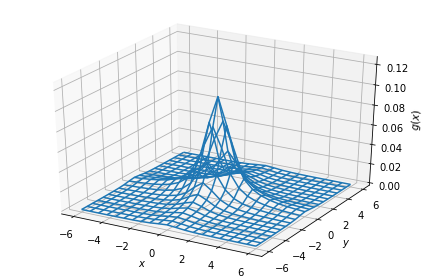
\includegraphics[width=0.5\linewidth]
		{figs/examplebvbmctrue.png}}
	\subfloat[Estimated density]{\label{fig11b}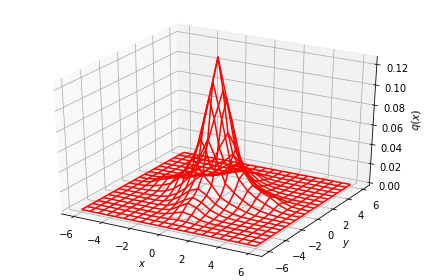
\includegraphics[width=0.5\linewidth]
		{figs/examplebvbmcestimated.png}}
\end{figure}
\end{block}
\end{frame}
% % % % % % % % % % % % % % % % % % % % % % % % % % % % % % % % 
\begin{frame}
\begin{block}{BVBMC package}
	Open source Python package, that can be found in \url{https://github.com/DFNaiff/BVBMC}. Still lacks documentation (to be fixed soon).
	
	Since it may (and probably will) undergo changes, code specific to this work can be found in \url{https://github.com/DFNaiff/Dissertation}.
\end{block}

\begin{block}{Implementation}
Implementation of BVBMC package is heavily dependent on PyTorch.

Due to the variety of inner optimizers, various gradient calculations are required. Automatic differentiation in PyTorch makes this process much more concise and less error prone.
\end{block}

\end{frame}
\section{Experiments}
\begin{frame}
\begin{block}{1-d mixture of Gaussians}
	\begin{figure}
		\centering
		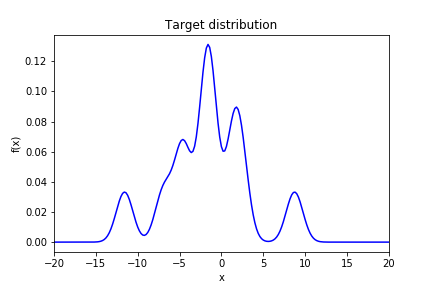
\includegraphics[width=0.6\linewidth]{figs/targetexil1a.png}
	\end{figure}
	\begin{displaymath}
	f(x) = \sum_{i=1}^{12} w_i \mathcal{N}(x;\mu_i,\sigma^2_i),
	\end{displaymath}
	\centering{$w_i = \frac{1}{12}$, $\mu_i \sim \mathcal{N}(0,\sqrt{5})$, $\sigma^2_i = 1$}.
\end{block}
\end{frame}

\begin{frame}
\begin{block}{Kernel performance}
\begin{figure}
	\centering
	\captionsetup[subfigure]{labelformat=empty}
	\subfloat[$k_{\text{PMat},5/2}$, moments.]{\label{fig11a}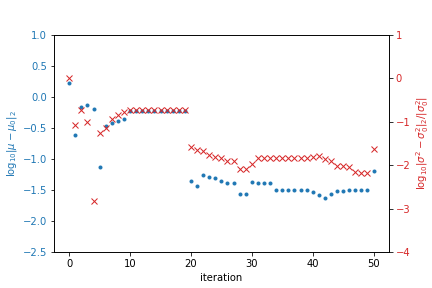
\includegraphics[width=0.5\linewidth]
		{figs/dmcil1fk52.png}}
	\subfloat[$k_{\text{PMat},5/2}$, final result.]{\label{fig11b}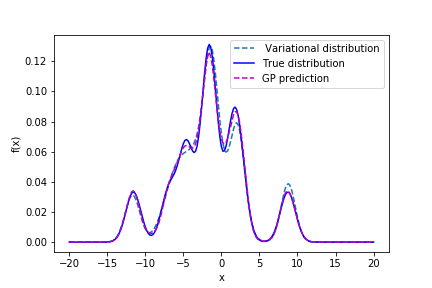
\includegraphics[width=0.5\linewidth]
		{figs/convgraphil1fk52.png}}
	

\end{figure}
\end{block}
\end{frame}

\begin{frame}
\begin{block}{Kernel performance}
	\begin{figure}
		\centering
		\captionsetup[subfigure]{labelformat=empty}
		
		\subfloat[$k_{\text{SQE}}$, moments.]{\label{fig11a}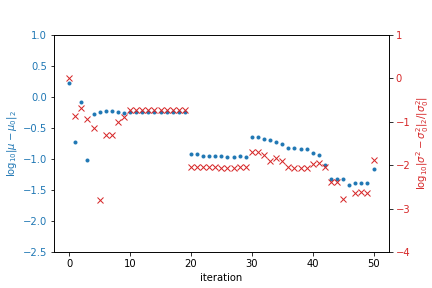
\includegraphics[width=0.5\linewidth]
			{figs/dmcil1fkSQE.png}}
		\subfloat[$k_{\text{SQE}}$, final result.]{\label{fig11b}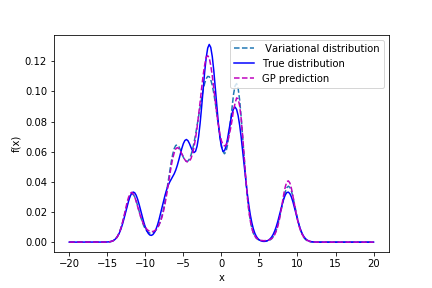
\includegraphics[width=0.5\linewidth]
			{figs/convgraphil1fkSQE.png}}
	\end{figure}
\end{block}
\end{frame}

\begin{frame}
\begin{block}{Training routine}
\begin{figure}
	\centering
	\captionsetup[subfigure]{labelformat=empty}
	\subfloat[Routine A, moments]{\label{fig11a}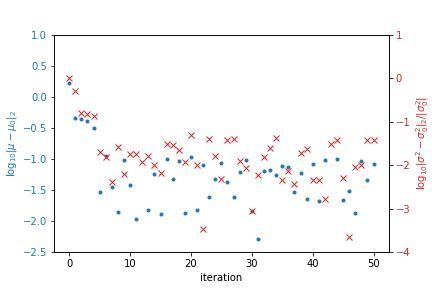
\includegraphics[width=0.5\linewidth]
		{figs/dmcil1ati1.png}}
	\subfloat[Routine A, running time.]{\label{fig11b}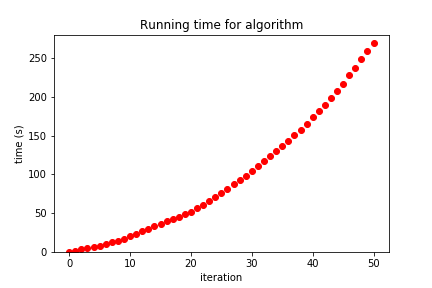
\includegraphics[width=0.5\linewidth]
		{figs/timegraphil1ati1.png}}

\end{figure}
\end{block}
\end{frame}

\begin{frame}
\begin{block}{Training routine}
	\begin{figure}
		\centering
		\captionsetup[subfigure]{labelformat=empty}
		
		\subfloat[Routine B,moments.]{\label{fig11a}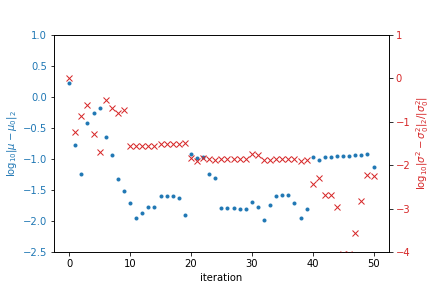
\includegraphics[width=0.5\linewidth]
			{figs/dmcil1ati10.png}}
		\subfloat[Routine B, running time.]{\label{fig11b}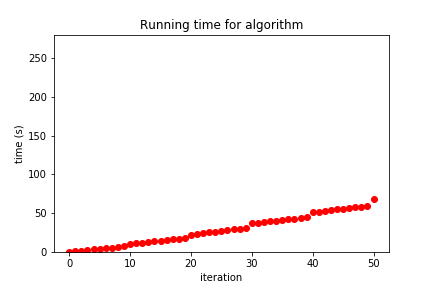
\includegraphics[width=0.5\linewidth]
			{figs/timegraphil1ati10.png}}
	\end{figure}
\end{block}
\end{frame}

\begin{frame}
\begin{block}{Training routine}
	\begin{figure}
		\centering
		\captionsetup[subfigure]{labelformat=empty}
		
		\subfloat[Routine C,moments.]{\label{fig11a}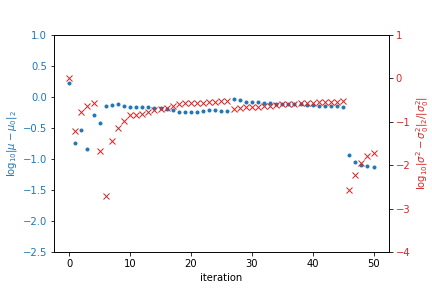
\includegraphics[width=0.5\linewidth]
			{figs/dmcil1ati1000.png}}
		\subfloat[Routine C, running time.]{\label{fig11b}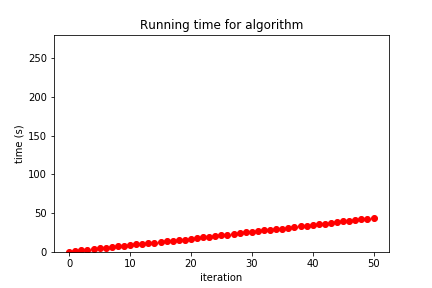
\includegraphics[width=0.5\linewidth]
			{figs/timegraphil1ati1000.png}}
	\end{figure}
\end{block}
\end{frame}

\begin{frame}
\begin{block}{Active evaluation}
\begin{figure}
	\centering
	\captionsetup[subfigure]{labelformat=empty}
	\subfloat[PROP, moments.]{\label{fig11a}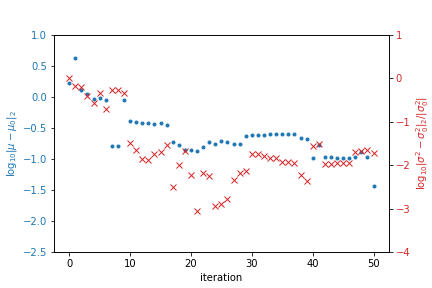
\includegraphics[width=0.5\linewidth]
		{figs/dmcil1g_aq_prospective.png}}
	\subfloat[PROP, sampling.]{\label{fig11b}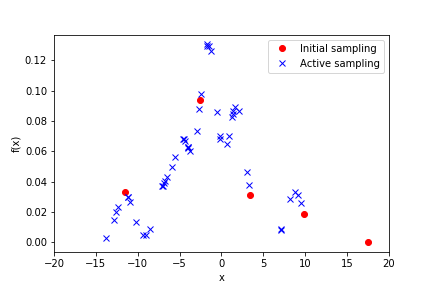
\includegraphics[width=0.5\linewidth]
		{figs/explopattern1g_aq_prospective.png}}

\end{figure}
\end{block}
\end{frame}

\begin{frame}
\begin{block}{Active evaluation}
	\begin{figure}
		\centering
		\captionsetup[subfigure]{labelformat=empty}
		
		\subfloat[MMLT, moments.]{\label{fig11a}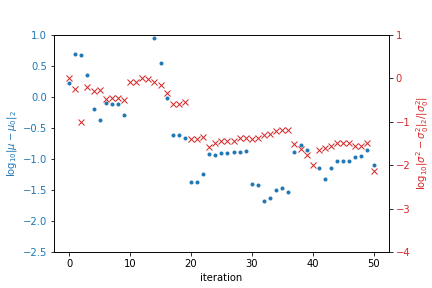
\includegraphics[width=0.5\linewidth]
			{figs/dmcil1g_aq_mmlt.png}}
		\subfloat[MMLT, sampling.]{\label{fig11b}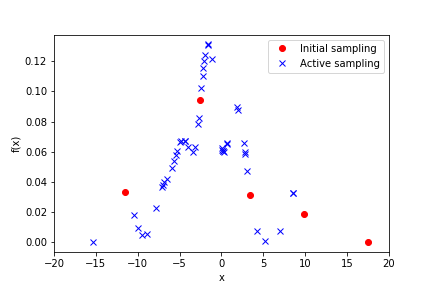
\includegraphics[width=0.5\linewidth]
			{figs/explopattern1g_aq_mmlt.png}}
		
	\end{figure}
\end{block}
\end{frame}

\begin{frame}
\begin{block}{N-d toy examples}
\begin{itemize}
	\item \textit{Lumpy}
	\begin{equation*}
	f(x) = \sum_{i=1}^{12} w_i \mathcal{N}(x;\mu_i,\Sigma_i),
	\end{equation*}
	$(w_1,\ldots,w_{12}) \sim \text{Dir}(1,\ldots,1)$, $\mu_i \sim \text{Unif}([0,1]^D)$, $\Sigma = \text{diag}(\sigma_1^2,\ldots,\sigma_n^2)$, $\sigma_i^2 \sim \text{Unif}(0.2,0.6)$.
	
	\item \textit{Cigar}
	\begin{equation*}
	f(x) = \mathcal{N}(x;0,\Sigma),
	\end{equation*}
	$\Sigma = Q \Lambda Q^T$, $\Lambda = (10.0,0.1,\ldots,0.1)$, $Q \sim \text{Unif}(SO(D))$.
	
	\item \textit{Student-t} 
	\begin{equation*}
	f(x) =  \prod_{d=1}^D \mathcal{T}(x_i;\nu_i),
	\end{equation*}
	$\nu_i \sim \text{Unif}(2.5,2+0.5D)$.
\end{itemize}
\end{block}
\end{frame}
\begin{frame}
\begin{block}{N-d toy examples}
For each case, dimensions $D = 2,6,10$ where tested, and the BVBMC algorithm was run for $100$ iterations, with $10D$ initial samples. The GP kernel used were $k_{\text{PMat},\nu=2.5}$, with active evaluation at each iteration, according to an acquisition function randomly chosen between the pair $(\alpha_\text{PROP},\alpha_\text{MMLT})$. Every 20 steps, joint parameter updating was done, and pruning was done at each iteration, with $\beta = 10^{-3}$.
\end{block}
\end{frame}
\begin{frame}
\begin{block}{Comparison with VBMC}
\begin{table}[]
\begin{tabular}{l|l|l|l|l|}
	\cline{2-5}
	& \multicolumn{2}{l|}{Lumpy} & \multicolumn{2}{l|}{Cigar} \\ \cline{2-5} 
	& BVBMC         & VBMC        & BVBMC         & VBMC 
	\\ 
	\hline
	\multicolumn{1}{|l|}{D=2}  & $3.12 \times 10^{-3}$        & $6.5 \times 10^{-4}$         & $8.12 \times 10^{-3}$           & $2.1 \times 10^{-1}$          \\ 
	\hline
	\multicolumn{1}{|l|}{D=6}  & $6.59 \times 10^{-2}$         & $ 3.5 \times 10^{-2}$         & $5.56 \times 10^{-1}$           & $ 1.07 \times 10^{-1}$        \\ \hline
	\multicolumn{1}{|l|}{D=10} & $1.19 \times 10^{-1}$           & $ 4.2 \times 10^{-1}$         & $1.29 $           &  $ 1.0 \times 10^{-1}$        \\ \hline
\end{tabular}

\begin{tabular}{l|l|l|}
	\cline{2-3}
	& \multicolumn{2}{l|}{Student-t} \\ \cline{2-3} 
	& BVBMC         & VBMC         \\ \hline
	\multicolumn{1}{|l|}{D=2} & $2.9 \times 10^{-1}$          & $2.0 \times 10^{-3}$         \\ \hline
	\multicolumn{1}{|l|}{D=6}     & $1.14 \times 10^{-1}$           & $2.3 \times 10^{-1}$         \\ \hline
	\multicolumn{1}{|l|}{D=10} & $2.56 \times 10^{-1}$           & $ 2.7 \times 10^{-1}$        \\ \hline
\end{tabular}

\end{table}
\end{block}
\end{frame}
\begin{frame}
\begin{block}{}
\begin{figure}
	\centering
	\captionsetup[subfigure]{labelformat=empty}
	\subfloat[Lumpy, means convergence.]{\label{fig11a}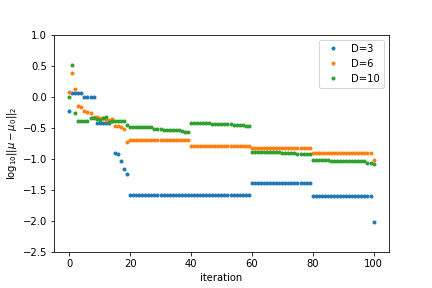
\includegraphics[width=0.5\linewidth]
		{figs/ex1b_mean.png}}
	\subfloat[Lumpy, covariances convergence.]{\label{fig11b}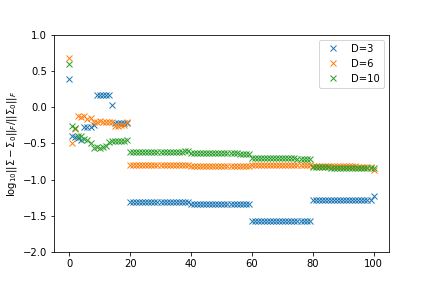
\includegraphics[width=0.5\linewidth]
		{figs/ex1b_cov.png}}

\end{figure}
\end{block}{}
\end{frame}

\begin{frame}
\begin{block}{}
	\begin{figure}
		\centering
		\captionsetup[subfigure]{labelformat=empty}
		
		\subfloat[Cigar, means convergence.]{\label{fig11a}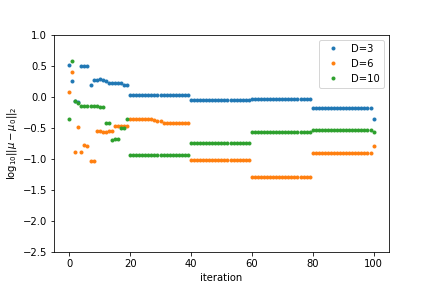
\includegraphics[width=0.5\linewidth]
			{figs/ex4b_mean.png}}
		\subfloat[Cigar, covariances convergence.]{\label{fig11b}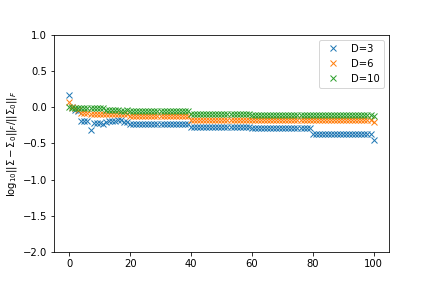
\includegraphics[width=0.5\linewidth]
			{figs/ex4b_cov.png}}
	\end{figure}
\end{block}{}
\end{frame}

\begin{frame}
\begin{block}{}
\begin{figure}
\centering
\captionsetup[subfigure]{labelformat=empty}
\subfloat[Student-t, means convergence.]{\label{fig11a}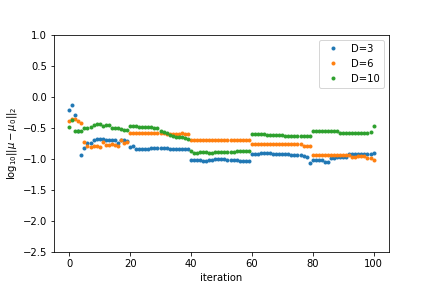
\includegraphics[width=0.5\linewidth]
	{figs/ex5b_mean.png}}
\subfloat[Student-t, covariances convergence.]{\label{fig11b}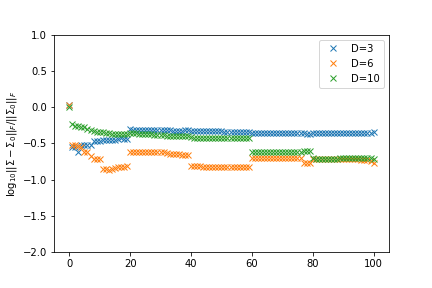
\includegraphics[width=0.5\linewidth]
	{figs/ex5b_cov.png}}
\end{figure}
\end{block}
\end{frame}
\begin{frame}
\begin{block}{Source problem}
\begin{equation*}
q(x,t) = q_0 \exp \left(-\frac{(x-x_0)^2}{2 \rho^2} \right) \mathbf{1}_{[0,t_s)}(t).
\end{equation*}
\begin{equation*}
\frac{\partial}{\partial t} u(x,t) = \frac{\partial^2}{\partial x^2} u(x,t) + q(x,t), \quad x \in (0,1).
\end{equation*}
\begin{equation*}
u(x,0) = 0, \; \frac{\partial}{\partial x} u(0,t) = \frac{\partial}{\partial x} u(1,t) = 0.
\end{equation*}
Objective: from measurements, estimate $(x_0,q_0,t_s,\rho)$.
\end{block}
\begin{block}{Likelihood model}
For $x_m=\{0,1\}$, measurements in $t_m \in \{0.075,0.15,0.225,0.3,0.4\}$.

$\mathcal{D} = \{\hat{u}(x_m,t_m)\}_{x_m \in \{0,1\},t_m \in T_m}$.

$\hat{u}(x_m,t_m) = u(x_m,t_m) + \epsilon$, $\epsilon \sim \mathcal{N}(0,\sigma^2)$, $\sigma^2 \sim \text{InvGamma}(\alpha,\beta)$.
\begin{equation*}
p(\mathcal{D}|x_0,t_s,q_0,\rho) = \prod_{x_m \in \{0,1\},t_m \in T_M} \mathcal{T}(\hat{u}(x_m,t_m);u(x_m,t_m),\beta/\alpha,2 \alpha).
\end{equation*}
\end{block}
\end{frame}
\begin{frame}
\begin{block}{Priors}
\begin{equation*}
\begin{split}
& p(x_0) = \text{Unif}(x_0;0,1) \\ 
& p(t_s) = \text{Unif}(t_s;0,0.4) \\
& p(q_0) = \text{HalfCauchy}(q_0;10) \\ 
& p(\rho) = \text{HalfCauchy}(\rho;0.1)
\end{split}
\end{equation*}
\end{block}

\begin{block}{Warped problem in $\mathbb{R}^4$}
\begin{equation*}
\begin{split}
& x_0 = \text{sigmoid}(\tilde{x}_0) \\
& t_s = 0.4 \times \text{sigmoid}(\tilde{t}_s) \\
& q_0 = \exp(\tilde{q}_0) \\
& \rho = \exp(\tilde{\rho}), \\
\end{split}
\end{equation*}
\begin{equation*}
\begin{split}
p(\tilde{x}_0,\tilde{t}_s,\tilde{q}_0,\tilde{\rho}|\mathcal{D}) \propto & p(x_0,q_0,t_s,\rho|\mathcal{D}) \times \\ & \text{sigmoid}'(\tilde{x}_0) \text{sigmoid}'(\tilde{t}_s) \exp(\tilde{q}_0) \exp(\tilde{\rho})
\end{split}
\end{equation*}
\end{block}
\end{frame}
\begin{frame}
\begin{block}{Problem generation}
A synthetic problem is considered with the true values being
\begin{equation*}
x_0,t_s,q_0,\rho = 0.230,0.300,6.366,0.050
\end{equation*}
The data was generated by solving the PDE by finite differences, and perturbing the measurements with by noise $\mathcal{N}(0,10^{-2})$.
\end{block}
\begin{block}{Parameter estimation}
	The likelihood is computed for each $x_0,t_s,q_0,\rho$ by computing $\hat{u}$ also by finite differences.
	
	The BVBMC algorithm is applied to the problem, with a total of 180 evaluations. It was compared to the EMCEE algorithm, used in astrophysics, and parameters are estimated by their posterior calculated means.
\end{block}
\end{frame}
\begin{frame}
\begin{block}{True values and estimations}
\begin{table}[h]
	\centering
	\begin{tabular}{l|l|l|l|l|}
		\cline{2-5}
		& $x_0$ & $t_s$ & $q_0$  & $\rho$ \\ \hline
		\multicolumn{1}{|l|}{True}  & 0.230 & 0.300 & 6.366  & 0.050  \\ \hline
		\multicolumn{1}{|l|}{BVBMC} & 0.328 & 0.213 & 5.435  & 0.140  \\ \hline
		\multicolumn{1}{|l|}{EMCEE} & 0.352 & 0.206 & 10.228 & 0.218  \\ \hline
	\end{tabular}
\end{table}
\end{block}
\end{frame}
\begin{frame}
\begin{block}{KDE for BVBMC solution}
\begin{figure}
	\centering
	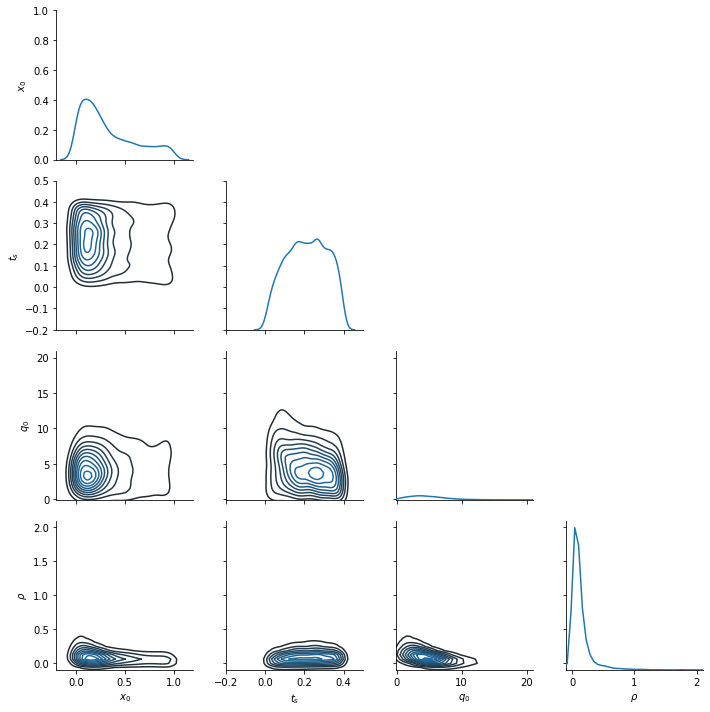
\includegraphics[width=0.6\linewidth]{figs/sourceproblemhistogramsvb.png}
\end{figure}
\end{block}
\end{frame}
\begin{frame}
\begin{block}{KDE for EMCEE solution}
	\begin{figure}
		\centering
		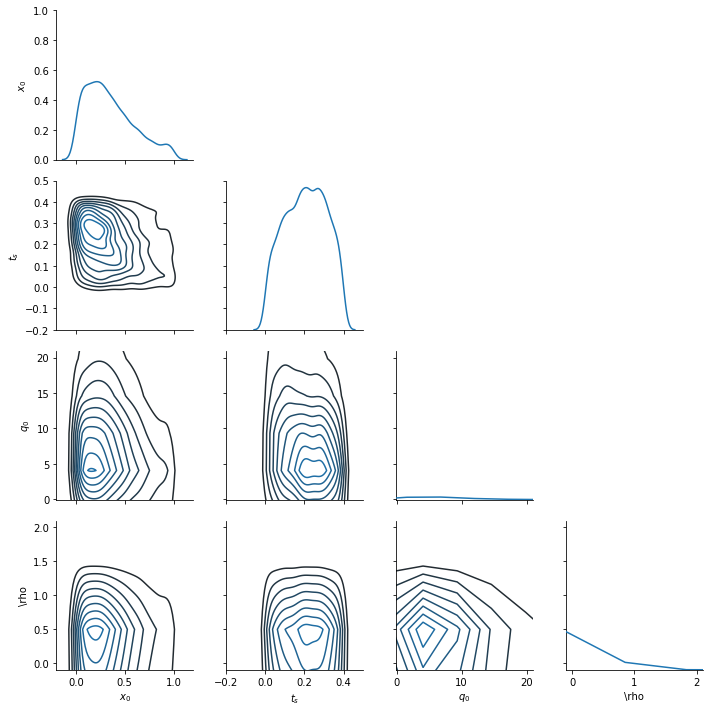
\includegraphics[width=0.6\linewidth]{figs/sourceproblemhistogramsemcee.png}
	\end{figure}
\end{block}
\end{frame}
\section{Challenges and conclusion}
\begin{block}{Challenges}
\begin{itemize}
	\item Boosted Variational Bayesian Monte Carlo is a "new" approach. As such, it remains to be seen in which cases it is best to use it.
	\item Posteriors in $\mathbb{R}^D$ are limited, and the warping approach is clumsy. How can BVBMC be extended to a larger class of domains? Probably the reparameterization trick will have to be used.
	\item How can this approach be extended do pseudo-marginals?
	\item Is there a way to incorporate Sparse Gaussian Process here? The author has tried to do this, although he wasn't successful.
\end{itemize}
\end{block}
\begin{block}{Conclusion}
The method presented in this work, although still immature, has shown promise for use in Bayesian inference, where the likelihood function is expensive of evaluate, that are common in inverse problems.

The associated package in \url{https://github.com/DFNaiff/BVBMC}, built on top of PyTorch, is intended to be easy to use, so a practitioner can quickly employ it in their own problems, if they wish so.

\end{block}
\end{document}
